

\section{Results} % (fold)
\label{sec:results}
The peaks of each measurement was recorded in Table~\ref{tab:dataCollected} and Figure~\ref{fig:Figures_aluminumShiftsPlot} and \ref{fig:Figures_plasticShiftsPlot} show the energy distributions from both absorbers while collecting data from $^{137}\text{Cs}$.
\begin{figure}[tbp]
	\centering
		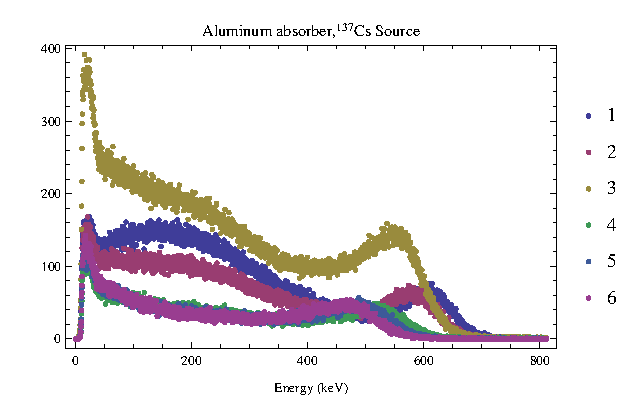
\includegraphics[width=.9\textwidth]{Figures/aluminumShiftsPlot.eps}
	\caption{The peaks also shift towards lower energies for aluminum. In order to normalize their intensities, the data for sheets 4,5, and 6 have a constraint on the maximum number of counts collected.  The numbers 1-6 in the plot above and 1-5,7 in Figure~\ref{fig:Figures_plasticShiftsPlot} represent the number of sheets between the radioactive isotope and the scintillator.}
	\label{fig:Figures_aluminumShiftsPlot}
\end{figure}%(fig:Figures_aluminumShiftsPlot)
\begin{figure}[tbp]
	\centering
		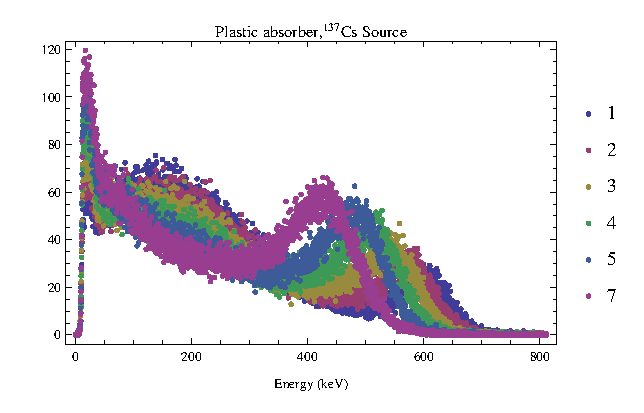
\includegraphics[width=.9\textwidth]{Figures/plasticShiftsPlot.eps}
	\caption{The peak of $^{137}\text{Cs}$ shifts towards lower energies as more absorbers are added.  The system was programmed to run until a set number of counts were collected.  The sum of three spectrums shown above contain: the beta spectrum of max energy $1175.63~\text{keV}$ (5\%), the beta spectrum of max energy $513.93~\text{keV}$ (95\%), and the gaussian distribution with a center at $624.3~\text{keV}$ (10\%).}
	\label{fig:Figures_plasticShiftsPlot}
\end{figure}%(fig:Figures_plasticShiftsPlot)
\begin{table}
	[tbp] 
	\begin{center}
		\begin{tabular}{lrrrr}
\toprule
 	 &  		\multicolumn{2}{c}{Aluminum} 			 & 			\multicolumn{2}{c}{Plastic} 				\\
\cmidrule(r){2-3}
\cmidrule(r){4-5}
n    & ($\text{peak}\pm\sigma$)~[keV] 	& Thickness (cm) & ($\text{peak}\pm\sigma$)~[keV] 	& Thickness (cm) 	\\
\midrule
0    & $624.259\pm3$					&	0	         &	$624.259\pm3$					&	0   			\\
1    & $601\pm4$						&	0.0054		 &	$591.5\pm6.5$					&	0.01			\\
2    & $577.5\pm1.5$					&	0.0108		 &	$567.5\pm5.5$					&	0.02			\\
3    & $550.5\pm7.5$					&	0.0162		 &	$537.5\pm6.5$					&	0.03			\\
4    & $505.5\pm1.5$					&	0.0216		 &	$501\pm9$						&	0.04			\\
5    & $470.5\pm8.5$					&	0.027	     &	$470.5\pm4.5$					&	0.05			\\
6    & $450.5\pm10.5$					&	0.0324		 &	\textit{N/A}					&	\textit{N/A}	\\
7    & 	\textit{N/A}	    			&	\textit{N/A} &	$413\pm13$						&	0.07  			\\
\bottomrule
		\end{tabular}
	\end{center}
	\caption{Data collected shows our estimated peaks with standard deviations from taking the average of two possible peaks, one low energy and one high energy.} \label{tab:dataCollected}
\end{table}%(tab:dataCollected)
The electron range, $R(E)$, is interpolated using a linear fit of thickness as a function of energy with the weights $1/\sigma^2$ from Table~\ref{tab:dataCollected}. We fit the function to the equation $R(E)=kE^B$, using a least squares fit.  We used a change of variables to transform our equation into a linear problem,
\begin{align*}
	\begin{matrix}
		y = m x + c 	 						\\
		\ln(R(E)) = y 	& 	\mathrm{d}y = \mathrm{d}R/R				\\
		\ln(E) = x 		& 	\mathrm{d}x = \mathrm{d}E/E				\\
		\ln(k) = c 		& 	\mathrm{d}c = \mathrm{d}k/k				\\
		B = m 			& 	\mathrm{d}m = \mathrm{d}B				\\
	\end{matrix}
\end{align*}


 Our chi-squared value for aluminum and plastic are $398$ and $33.4$ where $\text{N}-2 =5$.  For a good fit, we want $\chi^2\approx \text{N}-2$.  If $\chi^2 \gg \text{N}-2$, it suggests that we are either using the wrong function or our error bars are too small.  If $\chi^2 \ll \text{N}-2$, it suggests that the data fits so well that maybe our error bars are too large.\cite{garcia2000numerical}  We believe the function fit to our data sufficiently describes the range in this domain, but not outside of it.  
 The values for $k$ and $B$ of aluminium are obtained are: $k = \kaluminum \pm 0.001$ and $B = \Baluminum \pm 0.006$. The values for $k$ and $B$ of plastic are: $k = \kplastic \pm 0.002$ and $B = \Bplastic \pm 0.007$.  These error bars for aluminum and plastic are significantly too small, which also agrees with analysis of the chi-squared value.

 $R(E)$ has units of g/cm$^2$, making the values independent of the absorbing material. Figure~\ref{fig:Figures_alum_plas_NIST_plot} shows our results compared to two other credible sources\cite{RevModPhys.24.28,nistData}, each with uncertainties around 5\%.  

\begin{comment}
	\begin{figure}[tbp]
		\centering
			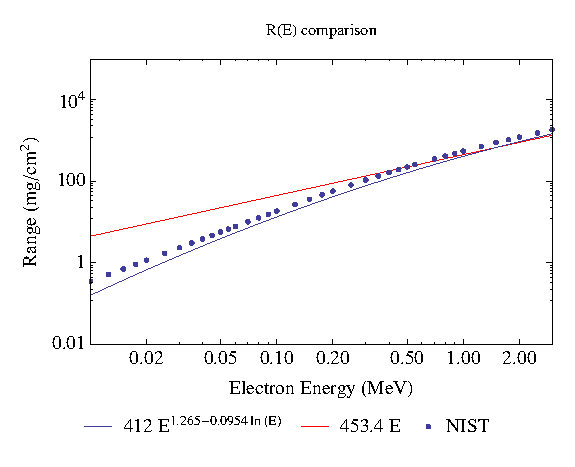
\includegraphics[width=.8\textwidth]{Figures/R_E_Comparison.eps}
		\caption{The data we collected agrees with those collected from different sources at higher energies and gets less accurate at lower energies.}
		\label{fig:Figures_R_E_Comparison}
	\end{figure}%fig:Figures_R_E_Comparison
\end{comment}

\begin{figure}[htbp]
  \centering 
  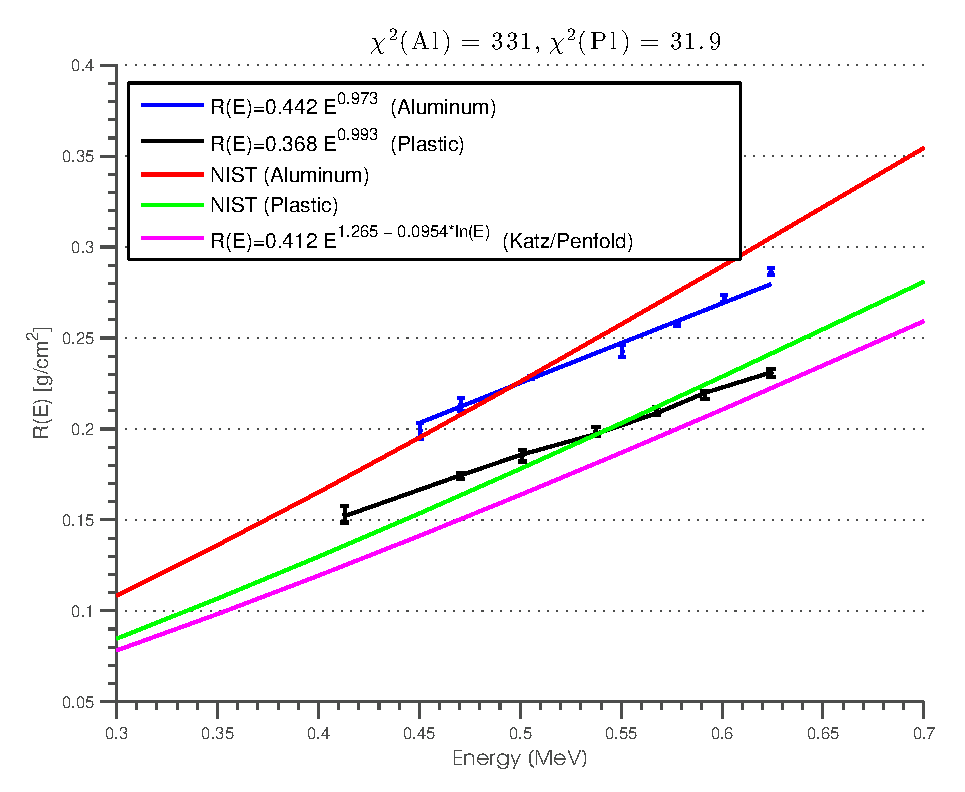
\includegraphics[width=\MyWidth]{Figures/alum_plas_NIST_plot.eps}
  \caption{Comparison of data from aluminum and plastic with accepted values.}
  \label{fig:Figures_alum_plas_NIST_plot}
\end{figure}%(fig:Figures_alum_plas_NIST_plot)


% section results (end)
